% $Id$
%
% Earth System Modeling Framework
% Copyright 2002-2013, University Corporation for Atmospheric Research,
% Massachusetts Institute of Technology, Geophysical Fluid Dynamics
% Laboratory, University of Michigan, National Centers for Environmental
% Prediction, Los Alamos National Laboratory, Argonne National Laboratory,
% NASA Goddard Space Flight Center.
% Licensed under the University of Illinois-NCSA License.


The ESMF Attribute class is a metadata utility that supports emerging standards 
in a flexible way.  The Attribute class is useful for documenting data 
provenance and encourages models to be more self describing.  Attributes can 
also be used to automate some aspects of model execution and coupling.

Metadata, which is data about data, is broken down into 
name-value pairs by the Attribute class.  Attributes can be attached at any 
level of the ESMF object hierarchy, and in some cases the Attributes of 
different ESMF objects can be linked together to form 
a corresponding Attribute hierarchy.  Attribute hierarchies are linked up
automatically for the most part, with the exception of links between Components 
and between a Component and a State.  Attribute hierarchies can also be 
unlinked, copied, and moved around as needed.

ESMF Attribute packages 
are used to aggregate, store, and output model metadata.  They can be 
nested inside each other to make larger organized packages, distributed across 
processors and updated at runtime, and expanded to suit specific needs.  The
ESMF-supplied  
Attribute packages are designed around accepted metadata conventions, such as: 
climate and forecast (CF) \cite{ref:cf}, ISO standards \cite{ref:iso}, and the METAFOR Common Information Model (CIM) \cite{ref:cim} \cite{ref:esdoccim}.

Most of the ESMF deep objects can host Attributes, and   
every object that can hold individual Attributes can also hold
Attribute packages.  Attribute hierarchies are supported for a majority of
the Attribute bearing classes.  
More information on the various Attribute 
capabilities, and the classes for which they are supported appear in the
following sections.

Reading Attribute XML files requires the Xerces C++ library, v3.1.0 
or better.  For more details, see the "ESMF Users Guide", "Building and 
Installing the ESMF, Third Party Libraries, Xerces".  Writing Attribute XML 
files is performed with the standard C++ output file stream facility.

\subsubsection{Schemas and Controlled Vocabularies}

There are two pieces to the information stored in Attributes.  One piece
is the property name and type, and its relation to other properties; this
is the schema.  The other piece is the range of values that are valid for
a particular property; this is the controlled vocabulary.  For many
information models, including the Common Information Model (CIM), these two
pieces are managed and versioned separately.

ESMF implements the appropriate schema internally; it translates the Attributes
as specified in the Attribute packages into the correct format based on the
convention and purpose as specified in arguments to most Attribute functions.
The controlled vocabularies, or Attribute values, however, are not controlled
or validated within ESMF.

\subsubsection{The Common Information Model (CIM)}

The CIM is a formal model of the climate modeling process being developed by
the European Union's \htmladdnormallink{METAFOR}{http://metaforclimate.eu/}
project.  The \htmladdnormallink{Earth System - Documentation (ES-DOC)}{http://earthsystemcog.org/projects/es-doc-models/} project
is an evolution of the METAFOR project, and they provide a detailed
description of the CIM \htmladdnormallink{here}{http://earthsystemcog.org/projects/es-doc-models/cim}.

ESMF is currently implementing only a subset of version 1.5 of the CIM, though this representation is expected to grow.

{\bf Mapping Attributes to the CIM}

The ESMF Attribute packages provide a structure for the Attributes that
are useful for climate modelers.  When the {\tt ESMF\_AttributeWrite()}
function is
called with "CIM" XML specified as the target, ESMF translates these package
structures into a format defined by the CIM schema.  The package descriptions
in the following sections provide a mapping from the ESMF Attribute name
to the CIM schema field.

For example, in the CIM Main Attribute Package, the Attribute named
"LongName" is mapped to the CIM schema field,
"software:SoftwareComponent:longName":

\begin{tabular}{|p{7cm}|p{5cm}|p{15mm}|p{15mm}|}
     \hline\hline
     {\bf Name} & {\bf Definition} & {\bf Controlled Vocabulary} & {\bf CIM Schema Field \linebreak (<CIM section>:<Entity>:<Field>)}\\
     \hline\hline
     {\tt LongName} & A version of the component name with all acronyms spelled out. & N/A & software:SoftwareComponent:longName \\
     \hline\hline
\end{tabular}
\linebreak

There are 3 parts to this mapping:

\begin{itemize}
  \item {\bf <CIM section>} = "software"
  \item {\bf <Entity>} = "SoftwareComponent"
  \item {\bf <Field>} = "longName"
\end{itemize}

The CIM section refers to the categories, or subsections, of the CIM
mentioned above.  In this example, the CIM section is "software".  To find
this section in the CIM schema repository, go to the
\htmladdnormallink{CIM repository}{http://metaforclimate.eu/trac/browser/CIM/tags/version-1.5/}
and then select the "software" drop down (see Figure \ref{fig:CIMRepository} ).

\begin{figure}[h]
\centering
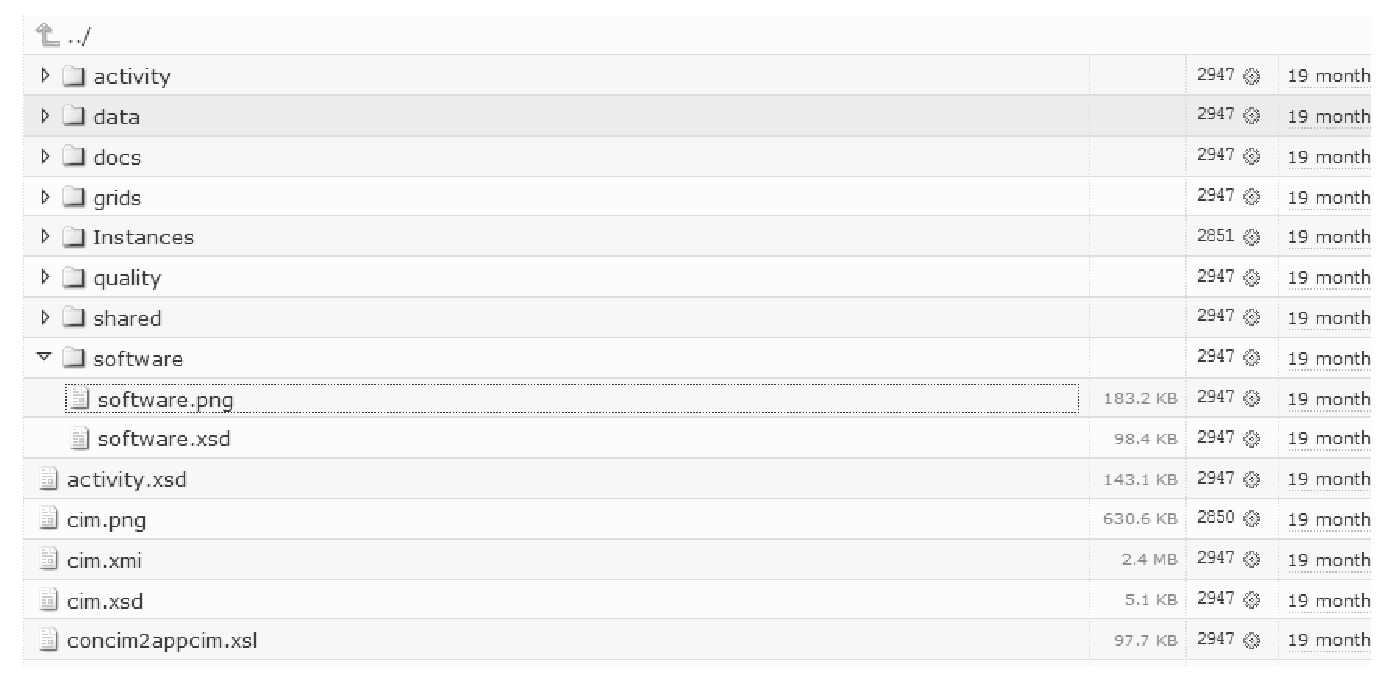
\includegraphics{CIMRepository}
\caption{The software section of the CIM repository}
\label{fig:CIMRepository}
\end{figure}
\clearpage

You can view the schema graphically in a UML diagram by selecting the
software.png file and then visually search the picture for the
SoftwareComponent entity.
However, this view does not provide field details, such as type and
description.  Alternatively, you can select the software.xsd file, and
then search the XML for the entity, "SoftwareComponent," and the field,
"longName," which will provide the details for this field (see Figure \ref{fig:LongNameXSD} ).

\begin{figure}[h]
\centering
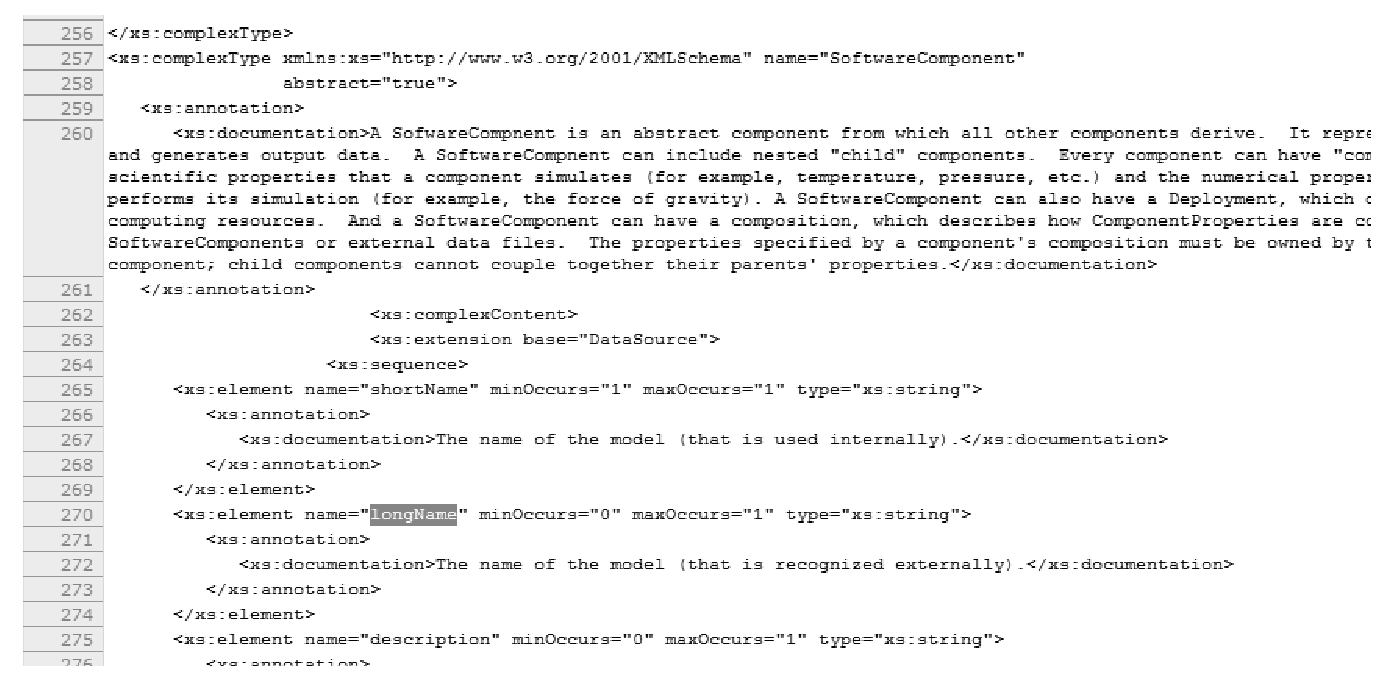
\includegraphics{LongNameXSD}
\caption{The longName Field in the CIM software XSD file}
\label{fig:LongNameXSD}
\end{figure}
\clearpage

As the ES-DOC team continues its work, more tools will be provided to support
CIM implementations.  Currently, a more user-friendly way to view the CIM
schema is available \htmladdnormallink{here}{http://es-doc.org/site/public/ontology}.


\subsubsection{The ESMF approach to Attributes}

ESMF's approach to Attributes can be summarized as follows:

\begin{itemize}
  \item Implement community standards where they exist.
  \item Associate Attributes with the ESMF object they describe. Currently, the following ESMF objects can have Attributes:
  \begin{itemize}
     \item CplComp
     \item GridComp
     \item State
     \item FieldBundle
     \item Field
     \item ArrayBundle
     \item Array
     \item Grid
     \item DistGrid
     \end{itemize}
  \item Establish pre-defined Attribute packages (see Section \ref{sec:AttPacks}) to make Attribute creation easier for the user.
  \item Allow for user-defined custom Attribute packages (see Section \ref{sec:CustomAttPacks}).
  \item Enable the nesting of Attribute packages (see Section \ref{sec:AttPackNesting}) including Custom packages.
  \item Enable complex Attribute hierarchies (see Section \ref{sec:AttHier}.
  \item Export Attributes in more than one format (see Section \ref{sec:AttributeExports}).
  \item Ensure that all Attributes are consistent across the entire virtual machine of the object to which they are attached.
\end{itemize}

\subsubsection{Attribute hierarchies}
\label{sec:AttHier}

Of the ESMF objects with Attributes, only some can link their Attributes together in an Attribute hierarchy.  These objects are:

\begin{itemize}
\item CplComp
\item GridComp
\item State
\item FieldBundle
\item Field
\item ArrayBundle
\item Array
\end{itemize}

Every ESMF deep object is given a {\tt root} Attribute on creation.
These {\tt root} Attributes serve as the attachment point for all metadata that 
is stored on a particular ESMF object, including all Attributes and
Attribute packages.  The {\tt root} Attributes can also be connected together via 
the {\tt ESMF\_AttributeLink()} functionality.  This happens automatically in most 
cases, such as when a Field is added to a FieldBundle, and results
in the formation of an Attribute hierarchy which mirrors the structure 
of the underlying object hierarchy.  

When two Attribute hierarchies are linked together 
the objects are given read-only access to each other's Attributes.
To ensure consistency across a distributed system, 
there can only ever be one set of Attributes associated with each ESMF object.  
This implies that a copy operation on an ESMF object Attribute hierarchy {\it can} 
use a value copy for all Attributes which are owned by the object being copied, 
but {\it must} use a reference copy for all Attributes which the object can 
access (through links) but does NOT own. See section \ref{sec:Att:Copy} for more
details on this concept.

The most common use for this hierarchy capability is for linking the Attributes 
of a Field to the FieldBundle which holds it, which is then linked to the 
State that is used to transport all of the data for a Component.  All of 
these links, with the exception of the link between the Component and the 
State, are automatically handled by ESMF. Additionally, the State will 
automatically set a {\tt VariableIntent} Attribute for Field when that Field 
is added to the State.  {\tt VariableIntent} will be set to either 
{\tt Export} or {\tt Import}.

